\newcommand{\colspacing}{\hspace{1.8em}}
\begin{table}[t]
\small
\centering
\setlength{\tabcolsep}{0.3em}
\caption{Program statistics and race-checking results from applying \whoop and \corral on our benchmarks.}
\label{tab:stats}
\begin{tabular}{l rrr rr r}
\centering
& & & & \multicolumn{2}{c}{\textbf{\whoop}}
& \textbf{\corral}\\
\cmidrule(lr){5-6}
\cmidrule(lr){7-7}

& & & & \multicolumn{1}{r}{\textbf{\#Racy}}
& \multicolumn{1}{r}{\textbf{\#Racy}}
& \multicolumn{1}{r}{\textbf{\#Races}}\\

\textbf{Benchmarks}
& \textbf{LoC}
& \textbf{\#Pairs}
& \textbf{\#MRs}
& \multicolumn{1}{r}{\textbf{Pairs}}
& \multicolumn{1}{r}{\textbf{MRs}}
& \multicolumn{1}{r}{\textbf{Found}}\\[0.3em]

\toprule

generic\_nvram
& 283
& 14
& 39
& \multicolumn{1}{r}{7}
& \multicolumn{1}{r}{2}
& 4\\

pc8736x\_gpio
& 354
& 27
& 55
& \multicolumn{1}{r}{13}
& \multicolumn{1}{r}{6}
& 5\\

machzwd
& 457
& 10
& 49
& \multicolumn{1}{r}{6}
& \multicolumn{1}{r}{3}
& 1\\

ssu100
& 568
& 7
& 27
& \multicolumn{1}{r}{\xmark}
& \multicolumn{1}{r}{\xmark}
& \xmark\\

intel\_scu\_wd
& 632
& 10
& 45
& \multicolumn{1}{r}{5}
& \multicolumn{1}{r}{1}
& 2\\

ds1286
& 635
& 15
& 49
& \multicolumn{1}{r}{5}
& \multicolumn{1}{r}{3}
& \xmark\\

dtlk
& 750
& 21
& 53
& \multicolumn{1}{r}{10}
& \multicolumn{1}{r}{6}
& \xmark\\

fs3270
& 883
& 15
& 54
& \multicolumn{1}{r}{9}
& \multicolumn{1}{r}{1}
& \xmark\\

gdrom
& 890
& 94
& 41
& \multicolumn{1}{r}{21}
& \multicolumn{1}{r}{2}
& \xmark\\

swim
& 996
& 28
& 80
& \multicolumn{1}{r}{15}
& \multicolumn{1}{r}{7}
& 8\\

intel\_nfcsim
& 1272
& 10
& 24
& \multicolumn{1}{r}{10}
& \multicolumn{1}{r}{2}
& \xmark\\

ps3vram
& 1499
& 4
& 32
& \multicolumn{1}{r}{1}
& \multicolumn{1}{r}{1}
& \xmark\\

sonypi
& 1729
& 30
& 62
& \multicolumn{1}{r}{19}
& \multicolumn{1}{r}{4}
& 2\\

sx8
& 1751
& 2
& 47
& \multicolumn{1}{r}{2}
& \multicolumn{1}{r}{1}
& 1\\

8139too
& 2694
& 46
& 37
& \multicolumn{1}{r}{40}
& \multicolumn{1}{r}{4}
& \xmark\\

r8169
& 7205
& 192
& 50
& \multicolumn{1}{r}{88}
& \multicolumn{1}{r}{1}
& \xmark\\

\bottomrule
\end{tabular}
\end{table}

\begin{table*}[t]
\small
\centering
\setlength{\tabcolsep}{0.45em}
\caption{Comparison with different yield instrumentation granularities and context-switch bounds.}
\label{tab:results}
\begin{tabular}{l r rrrr rrrr rrrr}
\centering
& \textbf{\whoop}
& \multicolumn{3}{c}{\textbf{\corral}}
& \multicolumn{6}{c}{\textbf{\whoop + \corral}}\\
\cmidrule(lr){2-2}
\cmidrule(lr){3-5}
\cmidrule(lr){6-11}

& \multirow{2}{*}{\textbf{Time}}
& \multicolumn{3}{c}{\textbf{\yieldall\xspace --- Time (sec)}}
& \multicolumn{3}{c}{\textbf{\yieldcoarse\xspace --- Time (sec)}}
& \multicolumn{3}{c}{\textbf{\yieldmr\xspace --- Time (sec)}}\\
\cmidrule(lr){3-5}
\cmidrule(lr){6-8}
\cmidrule(lr){9-11}

\textbf{Benchmarks}
& \textbf{\textbf{(sec)}}
& \multicolumn{1}{r}{\textbf{csb = 2}}
& \multicolumn{1}{r}{\textbf{csb = 5}}
& \multicolumn{1}{r}{\textbf{csb = 9}}
& \multicolumn{1}{r}{\textbf{csb = 2}}
& \multicolumn{1}{r}{\textbf{csb = 5}}
& \multicolumn{1}{r}{\textbf{csb = 9}}
& \multicolumn{1}{r}{\textbf{csb = 2}}
& \multicolumn{1}{r}{\textbf{csb = 5}}
& \multicolumn{1}{r}{\textbf{csb = 9}}\\[0.3em]

\toprule

generic\_nvram
& \multicolumn{1}{r}{2.7}
& \multicolumn{1}{r}{27.9}
& \multicolumn{1}{r}{38.4}
& \multicolumn{1}{r}{146.2}
& \multicolumn{1}{r}{17.6}
& \multicolumn{1}{r}{22.2}
& \multicolumn{1}{r}{90.8}
& \multicolumn{1}{r}{14.2}
& \multicolumn{1}{r}{16.5}
& \multicolumn{1}{r}{42.0}\\

pc8736x\_gpio
& \multicolumn{1}{r}{5.3}
& \multicolumn{1}{r}{145.6}
& \multicolumn{1}{r}{302.0}
& \multicolumn{1}{r}{}
& \multicolumn{1}{r}{89.5}
& \multicolumn{1}{r}{229.5}
& \multicolumn{1}{r}{}
& \multicolumn{1}{r}{41.7}
& \multicolumn{1}{r}{56.9}
& \multicolumn{1}{r}{426.6}\\

machzwd
& \multicolumn{1}{r}{}
& \multicolumn{1}{r}{}
& \multicolumn{1}{r}{}
& \multicolumn{1}{r}{}
& \multicolumn{1}{r}{}
& \multicolumn{1}{r}{}
& \multicolumn{1}{r}{}
& \multicolumn{1}{r}{}
& \multicolumn{1}{r}{}
& \multicolumn{1}{r}{}\\

ssu100
& \multicolumn{1}{r}{}
& \multicolumn{1}{r}{}
& \multicolumn{1}{r}{}
& \multicolumn{1}{r}{}
& \multicolumn{1}{r}{}
& \multicolumn{1}{r}{}
& \multicolumn{1}{r}{}
& \multicolumn{1}{r}{}
& \multicolumn{1}{r}{}
& \multicolumn{1}{r}{}\\

intel\_scu\_wd
& \multicolumn{1}{r}{}
& \multicolumn{1}{r}{}
& \multicolumn{1}{r}{}
& \multicolumn{1}{r}{}
& \multicolumn{1}{r}{}
& \multicolumn{1}{r}{}
& \multicolumn{1}{r}{}
& \multicolumn{1}{r}{}
& \multicolumn{1}{r}{}
& \multicolumn{1}{r}{}\\

ds1286
& \multicolumn{1}{r}{}
& \multicolumn{1}{r}{}
& \multicolumn{1}{r}{}
& \multicolumn{1}{r}{}
& \multicolumn{1}{r}{}
& \multicolumn{1}{r}{}
& \multicolumn{1}{r}{}
& \multicolumn{1}{r}{}
& \multicolumn{1}{r}{}
& \multicolumn{1}{r}{}\\

dtlk
& \multicolumn{1}{r}{}
& \multicolumn{1}{r}{}
& \multicolumn{1}{r}{}
& \multicolumn{1}{r}{}
& \multicolumn{1}{r}{}
& \multicolumn{1}{r}{}
& \multicolumn{1}{r}{}
& \multicolumn{1}{r}{}
& \multicolumn{1}{r}{}
& \multicolumn{1}{r}{}\\

fs3270
& \multicolumn{1}{r}{}
& \multicolumn{1}{r}{}
& \multicolumn{1}{r}{}
& \multicolumn{1}{r}{}
& \multicolumn{1}{r}{}
& \multicolumn{1}{r}{}
& \multicolumn{1}{r}{}
& \multicolumn{1}{r}{}
& \multicolumn{1}{r}{}
& \multicolumn{1}{r}{}\\

gdrom
& \multicolumn{1}{r}{}
& \multicolumn{1}{r}{}
& \multicolumn{1}{r}{}
& \multicolumn{1}{r}{}
& \multicolumn{1}{r}{}
& \multicolumn{1}{r}{}
& \multicolumn{1}{r}{}
& \multicolumn{1}{r}{}
& \multicolumn{1}{r}{}
& \multicolumn{1}{r}{}\\

swim
& \multicolumn{1}{r}{}
& \multicolumn{1}{r}{}
& \multicolumn{1}{r}{}
& \multicolumn{1}{r}{}
& \multicolumn{1}{r}{}
& \multicolumn{1}{r}{}
& \multicolumn{1}{r}{}
& \multicolumn{1}{r}{}
& \multicolumn{1}{r}{}
& \multicolumn{1}{r}{}\\

intel\_nfcsim
& \multicolumn{1}{r}{}
& \multicolumn{1}{r}{}
& \multicolumn{1}{r}{}
& \multicolumn{1}{r}{}
& \multicolumn{1}{r}{}
& \multicolumn{1}{r}{}
& \multicolumn{1}{r}{}
& \multicolumn{1}{r}{}
& \multicolumn{1}{r}{}
& \multicolumn{1}{r}{}\\

ps3vram
& \multicolumn{1}{r}{}
& \multicolumn{1}{r}{}
& \multicolumn{1}{r}{}
& \multicolumn{1}{r}{}
& \multicolumn{1}{r}{}
& \multicolumn{1}{r}{}
& \multicolumn{1}{r}{}
& \multicolumn{1}{r}{}
& \multicolumn{1}{r}{}
& \multicolumn{1}{r}{}\\

sonypi
& \multicolumn{1}{r}{}
& \multicolumn{1}{r}{}
& \multicolumn{1}{r}{}
& \multicolumn{1}{r}{}
& \multicolumn{1}{r}{}
& \multicolumn{1}{r}{}
& \multicolumn{1}{r}{}
& \multicolumn{1}{r}{}
& \multicolumn{1}{r}{}
& \multicolumn{1}{r}{}\\

sx8
& \multicolumn{1}{r}{}
& \multicolumn{1}{r}{}
& \multicolumn{1}{r}{}
& \multicolumn{1}{r}{}
& \multicolumn{1}{r}{}
& \multicolumn{1}{r}{}
& \multicolumn{1}{r}{}
& \multicolumn{1}{r}{}
& \multicolumn{1}{r}{}
& \multicolumn{1}{r}{}\\

8139too
& \multicolumn{1}{r}{}
& \multicolumn{1}{r}{}
& \multicolumn{1}{r}{}
& \multicolumn{1}{r}{}
& \multicolumn{1}{r}{}
& \multicolumn{1}{r}{}
& \multicolumn{1}{r}{}
& \multicolumn{1}{r}{}
& \multicolumn{1}{r}{}
& \multicolumn{1}{r}{}\\

r8169
& \multicolumn{1}{r}{228.1}
& \multicolumn{1}{r}{T.O.}
& \multicolumn{1}{r}{T.O.}
& \multicolumn{1}{r}{T.O.}
& \multicolumn{1}{r}{28755.2}
& \multicolumn{1}{r}{T.O.}
& \multicolumn{1}{r}{T.O.}
& \multicolumn{1}{r}{26939.4}
& \multicolumn{1}{r}{T.O.}
& \multicolumn{1}{r}{T.O.}\\

\bottomrule
\end{tabular}
\end{table*}

\begin{figure}
\centering
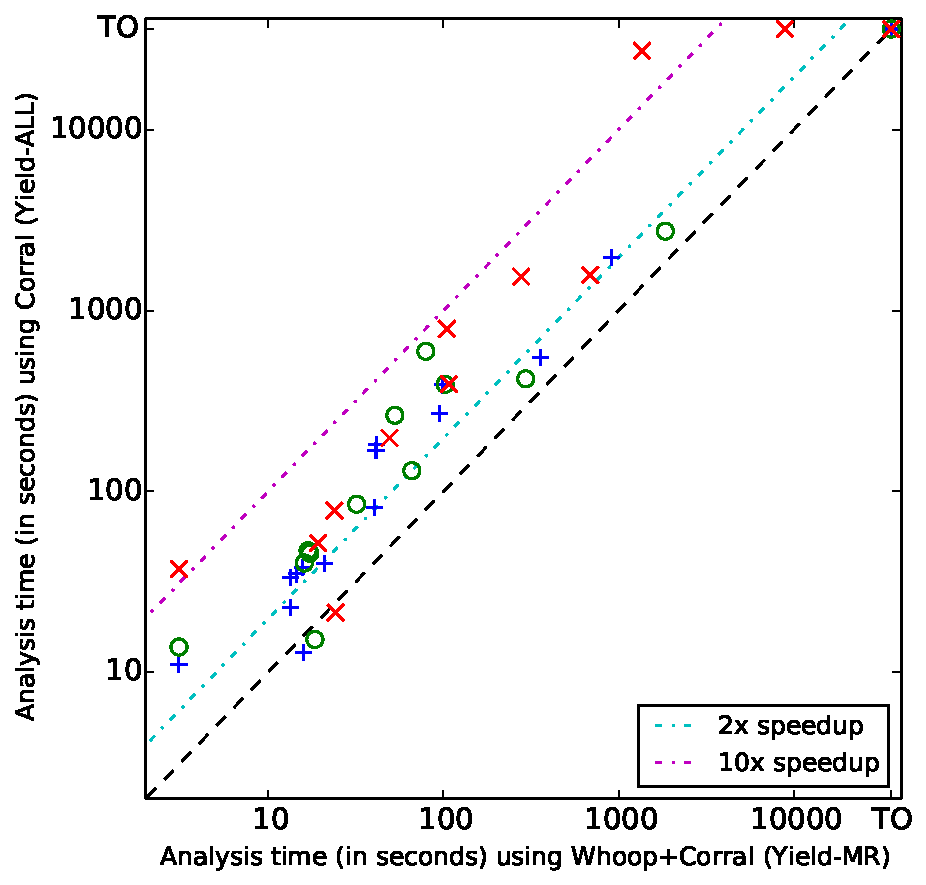
\includegraphics[width=.99\linewidth]{experiments/figures/yieldmr_vs_yieldall.pdf}
\caption{Scatter plot showing the runtime speedups that \corral achieves using \whoop with the \yieldmr instrumentation. The symbols $+$, $\circ$ and $\times$, represent a context-switch bound of 2, 5 and 9, respectively.}
\label{fig:plot}
\end{figure}

We performed experiments to validate the usefulness of the \whoop approach (Section~\ref{whoop}) and its combination with \corral (Section~\ref{corral}). We first present race-checking results from running \whoop and \corral on \sizeOfBenchmarks drivers taken from the 4.0 Linux kernel distribution.\footnote{\url{https://www.kernel.org}} We then evaluate the runtime performance and scalability of \corral and \whoop + \corral with different yield instrumentation granularities and context-switch bounds.
Our results demonstrate that \whoop can efficiently accelerate race-checking with \corral.

\medskip\noindent\textbf{Experimental Setup }
%
We performed all experiments on a 3.40GHz Intel Core i7-2600 CPU with 16GB RAM running Ubuntu Linux 12.04.5 LTS, LLVM 3.5, SMACK 1.5, Z3~4.3.2, Boogie rev. 4192 and \corral rev. 534. We also used Mono~4.1.0 to run Boogie and \corral.

\medskip\noindent\textbf{Benchmarks }
%
We evaluate our methodology against \sizeOfBenchmarks drivers taken from the 4.0 Linux kernel. We chose non-trivial drivers from several categories: block; char; ethernet; near field communication (nfc); universal serial bus (usb); and watchdog. We had to manually model the environment for these drivers, a process that required approximately two months of work.

\medskip\noindent\textbf{Race-Checking }
%
Table~\ref{tab:stats} presents statistics for all our benchmarks: lines of code (LoC); number of entry point pairs (\#Pairs); number of SMACK memory regions (\#MRs); number of potentially racy pairs identified by \whoop (\#Racy Pairs); number of potentially racy memory regions reported by \whoop (\#Racy MRs); and number of races discovered by \corral using a context-switch bound of 2 (\#Races Found). We did not discover new races with larger context-switch bounds. This might mean that these drivers only have races that manifest with at least one or two context-switches, or that \corral hit its bounds before discovering a deeper race.

We can see that \whoop reports more races than \corral. This is expected, since \whoop employs an over-approximating shared state abstraction to conservatively model the effects of additional threads when analyzing an entry point pair, and because lockset analysis is inherently imprecise; both factors can lead to false alarm race reports.  On the other hand, \corral is precise, but can miss races because only a limited number of context switches are considered.  Another issue with \corral is loop coverage due to unsound loop unrolling. To tackle this, we enable the built-in loop over-approximation described in~\cite{lal2014powering}. This can potentially lead \corral to report false positives, but we have not seen this in practice. Finally, when we apply \corral to a pair of entry points, we are just checking the specific pair and are not accounting for the effect of other threads (see Section~\ref{corral}); this can also cause \corral to miss some races.

Most of the races that \whoop and \corral discovered can be classified in two cases. The first case is accessing a global counter (or flag) from concurrent entry points, without a lock. This might be for performance, and indeed a lot of the races we found might be benign. Even benign races, though, lead to undefined behavior according to the C standard, and it is well known that undefined behaviors can lead to unexpected results when combined with aggressive compiler optimizations. The second case is an entry point accessing a field of an object (either global or passed as a parameter) without a lock. This can lead to a race if another entry point simultaneously accesses the same field of the same object.

As an example of the second case, we found the following race in the generic\_nvram char driver (see Figure~\ref{fig:data_race_example} for the source code): during the \texttt{llseek} entry point, the driver is accessing the file offset \texttt{file->f\_pos} without first acquiring a lock (\texttt{file} is passed as a parameter to \texttt{llseek}). This can lead to a race if the driver invokes \texttt{llseek} from another thread passing the same \texttt{file} object as a parameter. When we investigated another char driver that uses the same APIs, we saw that it was protecting the offset access in its \texttt{llseek} entry point with a mutex. This made us suspicious that the race we found in generic\_nvram could be real. We filed a bug report, but did not manage to get a response yet.

\medskip\noindent\textbf{Granularity of Context-Switches }
%
Table~\ref{tab:results} presents runtime results from using \whoop, \corral and \whoop + \corral to analyze our benchmarks, while Figure~\ref{fig:plot} plots the runtime speedups that \corral achieves using \whoop with the \yieldmr instrumentation. All reported times, in seconds, are averages over three runs. \corral was given a time budget of 10 hours (T.O. denotes timeout), and we considered context-switch bounds (csb) of 2, 5 and 9, respectively. When we run standalone \corral we enable the \yieldall instrumentation, which instruments context-switches (i.e. \texttt{yield} statements) after all visible operations. \whoop + \corral, instead, uses two different context-switch instrumentation granularities, \yieldcoarse and \yieldmr (see Section~\ref{corral}).

A higher context-switch bound results into deeper interleavings being explored and thus a larger sequentialized program. Intuitively, this means that we see even greater speedups using information from \whoop, when exploring deeper interleavings.

We can notice that \whoop is significantly faster than \corral. This is expected as \whoop achieves scalability using over-approximation and summarization techniques. This allows \whoop to perform especially well in complex drivers such as the r8169 ethernet driver: although \corral ... and timeouts with a csb of 9, \whoop manages to analyze the driver in 228.1 seconds. We believe that the reason behind this is that r8169 has many loops and uses deeply-nested recursion in some entry points, which \corral might not be able to handle efficiently.

%When \corral on its own tries to analyze the machzwd watchdog driver it explodes, because in some entry point pairs it attempts to analyze a large number of memory regions. For example for the entry point pair write vs init, it instruments interleavings at 26 different memory regions in a single invocation of \corral, which required approximately 1000 seconds to analyze. The same entry point pair is found race-free by \whoop. Using this information in \corral with the \yieldmr instrumentation, the pair takes less than a second to analyze. The \yieldcoarse instrumentation does not perform as well, because it works in the binary granularity of racy or non-racy entry points.
